\documentclass[a4paper,12pt]{article}
\usepackage[utf8]{inputenc}
\usepackage[german]{babel}
\usepackage{amsmath}
\usepackage{amssymb}
\usepackage{amsthm}
\usepackage{geometry}
\usepackage{graphicx}
\usepackage[hidelinks]{hyperref}
\usepackage{listings}
\usepackage{xcolor}
\usepackage{microtype}
\usepackage{enumitem}
\usepackage{booktabs}
\usepackage{tikz}
\usetikzlibrary{arrows.meta,positioning,shapes.geometric}

\geometry{margin=2.5cm}
\sloppy

\theoremstyle{definition}
\newtheorem{definition}{Definition}
\newtheorem{beispiel}{Beispiel}
\newtheorem{satz}{Satz}
\newtheorem{lemma}{Lemma}
\newtheorem{korollar}{Korollar}
\newtheorem{bemerkung}{Bemerkung}
\newtheorem{theorem}{Theorem}

\setlist[itemize,1]{label=--}

\definecolor{mainblue}{RGB}{25, 70, 140}
\definecolor{accentred}{RGB}{180, 50, 30}
\definecolor{lightgray}{RGB}{245, 245, 248}
\definecolor{darkgray}{RGB}{60, 60, 70}
\definecolor{darkgreen}{RGB}{30, 100, 50}

\hypersetup{
    colorlinks=true,
    linkcolor=mainblue,
    citecolor=accentred,
    urlcolor=mainblue,
    pdftitle={Python-AST-Konstruktion, Vergleich und Verifikation via Subgraph Algorithmus},
    pdfauthor={Stephan Epp},
}

\lstset{
    basicstyle=\ttfamily\small,
    keywordstyle=\color{blue},
    commentstyle=\color{gray},
    stringstyle=\color{accentred},
    numbers=left,
    numberstyle=\tiny,
    breaklines=true,
    columns=flexible,
    frame=single,
    literate=%
    {Ö}{{\"O}}1 {Ä}{{\"A}}1 {Ü}{{\"U}}1
    {ß}{{\ss}}1 {ü}{{\"u}}1 {ä}{{\"a}}1 {ö}{{\"o}}1
}

\lstdefinestyle{pystyle}{
    language=Python,
    morekeywords={ast,walk,dump,parse,NodeVisitor,visit,
                  NodeTransformer,fix_missing_locations},
    keywordstyle=\color{mainblue}\bfseries,
}

\title{\textbf{Python-AST-Konstruktion, Vergleich und\\
Verifikation via Subgraph Algorithmus}\\[0.1em]
\large Formale Grundlagen, Algorithmen und Ausblick}
\author{Stephan Epp}
\date{23. Juni 2026}

\begin{document}
\maketitle
\tableofcontents
\newpage

%=============================================================
\section{Einf\"uhrung}
%=============================================================

Der \emph{Abstract Syntax Tree} (AST) ist die kanonische interne
Repr\"asentation eines Python-Programms nach dem Parsing-Schritt.
Das CPython-Modul \texttt{ast} (Python~3.12) erzeugt, traversiert
und transformiert ASTs direkt aus Quellcode.  Jeder AST ist ein
gerichteter, gewurzelter Baum -- und damit ein spezieller gerichteter
Graph -- dessen Knoten syntaktische Konstrukte (Ausdr\"ucke,
Anweisungen, Bezeichner) und dessen Kanten die syntaktische
Eltern-Kind-Beziehung repr\"asentieren.

Diese Arbeit untersucht drei eng verwandte Fragestellungen:
\begin{enumerate}
    \item \textbf{Konstruktion:} Wie wird aus Python-Quellcode ein
          AST-Graph aufgebaut, und welche graphentheoretischen
          Eigenschaften hat er?
    \item \textbf{Vergleich:} Wie k\"onnen zwei Python-ASTs strukturell
          verglichen werden -- unter Abstraktion von Bezeichnernamen,
          Kommentaren und Formatierung?
    \item \textbf{Verifikation:} Wie l\"asst sich mit dem Subgraph
          Algorithmus (Epp~2026) \cite{epp2026} nachweisen, dass ein
          Programm eine Teilstruktur eines anderen enth\"alt
          (Subgraph-Isomorphismus)?
\end{enumerate}

Wir zeigen, dass der Subgraph Algorithmus f\"ur alle drei
Aufgaben eine effiziente, formal korrekte und gegen
oberfl\"achliche Code-Transformationen robuste L\"osung bietet
-- insbesondere bei der Plagiats\-erkennung, der Refactoring-
Verifikation und der Sicherheitsanalyse von Python-Code.

\subsection{Beitrag dieser Arbeit}

\begin{itemize}
    \item Formale Definition des Python-AST als gerichteter Graph
          $G_{\mathrm{AST}}$ mit Adjazenzmatrix und Signatur-Array.
    \item Polynomielle Reduktion des AST-Vergleichsproblems auf das
          Subgraph-Isomorphismusproblem.
    \item Vollst\"andige Korrektheits- und Laufzeitbeweise.
    \item Python-Implementierung des Subgraph Algorithmus auf ASTs.
    \item 12 empirische Visualisierungen (matplotlib).
    \item Ausf\"uhrlicher Ausblick auf zuk\"unftige Anwendungen.
\end{itemize}

\subsection{\"Uberblick der Reduktionen}

\begin{table}[ht]
\centering
\renewcommand{\arraystretch}{1.3}
\begin{tabular}{|l|l|c|}
\hline
\textbf{Problem} & \textbf{Graphmodell} & \textbf{Abschnitt}\\
\hline
AST-Konstruktion        & Gerichteter Baum $G_{\mathrm{AST}}$   & \ref{sec:konstr}\\
AST-Vergleich           & Signatur-Match via LCS                & \ref{sec:vergl}\\
AST-Verifikation (SI)   & Subgraph-Isomorphismus                & \ref{sec:verif}\\
Plagiats\-erkennung     & Subgraph-Einbettung                   & \ref{sec:plagiat}\\
Refactoring-Pr\"ufung   & Isomorphie-Test                       & \ref{sec:refact}\\
\hline
\end{tabular}
\caption{\"Ubersicht der behandelten Probleme und ihrer Graphmodelle}
\label{tab:uebersicht}
\end{table}

%=============================================================
\section{Grundlagen}
%=============================================================

\subsection{Definitionen}

\begin{definition}[Graph]
Ein \emph{gerichteter Graph} $G = (V, E)$ besteht aus einer
Knotenmenge $V = \{v_1, \ldots, v_n\}$ und einer Kantenmenge
$E \subseteq V \times V$.  Ein \emph{gewurzelter gerichteter Baum}
ist ein gerichteter Graph, bei dem genau ein Knoten $r \in V$
(die \emph{Wurzel}) keinen Eingangsknoten hat und jeder andere
Knoten genau einen Eingangsknoten besitzt.
\end{definition}

\begin{definition}[Adjazenzmatrix]
Die \emph{Adjazenzmatrix} $A \in \{0,1\}^{n \times n}$ eines
Graphen $G$ mit $n$ Knoten ist definiert durch
\[
A_{ij} = \begin{cases}
1 & \text{falls } (v_i, v_j) \in E,\\
0 & \text{sonst.}
\end{cases}
\]
\end{definition}

\begin{definition}[Subgraph]
$G = (V, E)$ ist ein \emph{Subgraph} von $G' = (V', E')$
(geschrieben $G \subseteq G'$), falls $V \subseteq V'$ und
$E \subseteq E'$.  Ein \emph{induzierter Subgraph} $G'[S]$
f\"ur $S \subseteq V'$ enth\"alt alle Kanten von $G'$ zwischen
Knoten in $S$.
\end{definition}

\begin{definition}[Subgraph-Isomorphismus]
\label{def:si}
Ein \emph{Subgraph-Isomorphismus} von $G$ nach $G'$ ist eine
injektive Abbildung $f\colon V \to V'$ mit
$(u, v) \in E \Rightarrow (f(u), f(v)) \in E'$.
\end{definition}

\begin{definition}[Zyklische Rotation]
Eine \emph{zyklische Rotation} einer Sequenz
$S = [s_0, s_1, \ldots, s_{n-1}]$ um $k$ Positionen ist
\[
\mathrm{rot}_k(S) = [s_k, s_{k+1}, \ldots, s_{n-1}, s_0, \ldots, s_{k-1}].
\]
\end{definition}

\begin{definition}[Subgraph Algorithmus (Epp~2026)]
\label{def:subgraph}
Der \emph{Subgraph Algorithmus} bestimmt f\"ur zwei Graphen
$G, G'$ mit je $n$ Knoten in Zeit $O(n^3)$ durch
Signatur-Arrays und zyklische Rotation, ob
$G \subseteq G'$, $G' \subseteq G$, $G = G'$ oder keiner
im anderen enthalten ist.
\end{definition}

\subsection{Python-AST: Grundstruktur}

Das CPython-Modul \texttt{ast} (Python~3.12) stellt 72 Knotentypen
bereit, aufgeteilt in sechs Kategorien
(Abbildung~\ref{fig:knotentypen}):

\begin{itemize}
    \item \textbf{Ausdr\"ucke} (\texttt{expr}): 28 Typen --
          \texttt{BinOp}, \texttt{Call}, \texttt{Name},
          \texttt{Attribute}, \texttt{Subscript}, \ldots
    \item \textbf{Anweisungen} (\texttt{stmt}): 19 Typen --
          \texttt{FunctionDef}, \texttt{ClassDef}, \texttt{If},
          \texttt{For}, \texttt{While}, \texttt{Return}, \ldots
    \item \textbf{Muster} (\texttt{pattern}): 12 Typen f\"ur
          \texttt{match}-Anweisungen (Python~3.10+).
    \item \textbf{Modulebene} (\texttt{mod}): 4 Typen --
          \texttt{Module}, \texttt{Interactive}, \texttt{Expression},
          \texttt{FunctionType}.
    \item \textbf{Typ-Ignorierungen} (\texttt{type\_ignore}):
          2 Typen.
    \item \textbf{Sonstige}: 7 Hilfstypen.
\end{itemize}

\begin{figure}[ht]
\centering
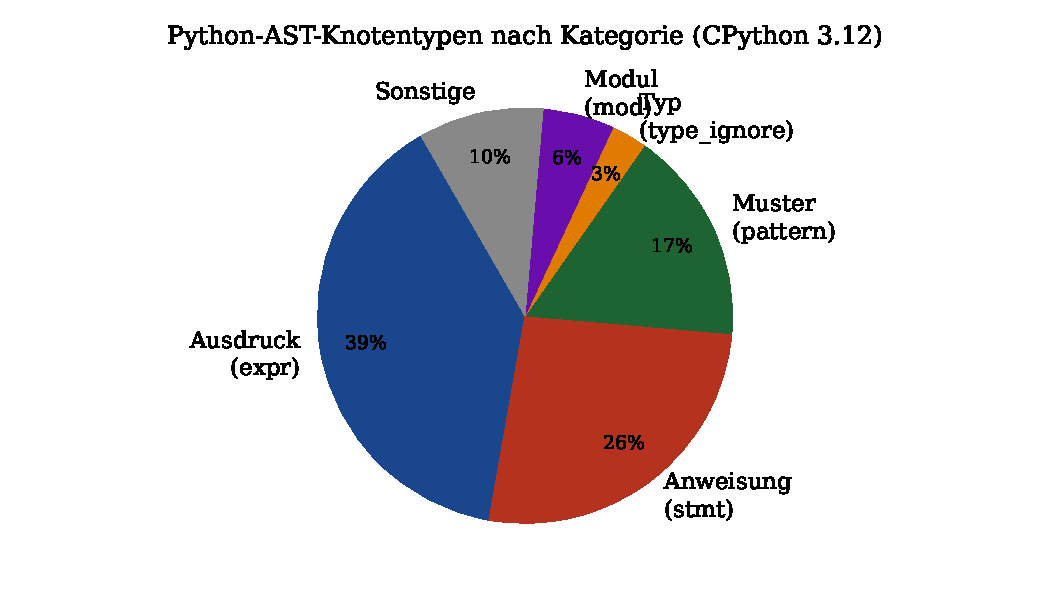
\includegraphics[width=0.80\textwidth]{plot1_ast_knotentypen.pdf}
\caption{Python-AST-Knotentypen nach Kategorie (CPython~3.12,
insgesamt 72 Typen).  Ausdr\"ucke und Anweisungen dominieren;
die Muster-Kategorie wurde mit Python~3.10 eingef\"uhrt.}
\label{fig:knotentypen}
\end{figure}

\begin{figure}[ht]
\centering
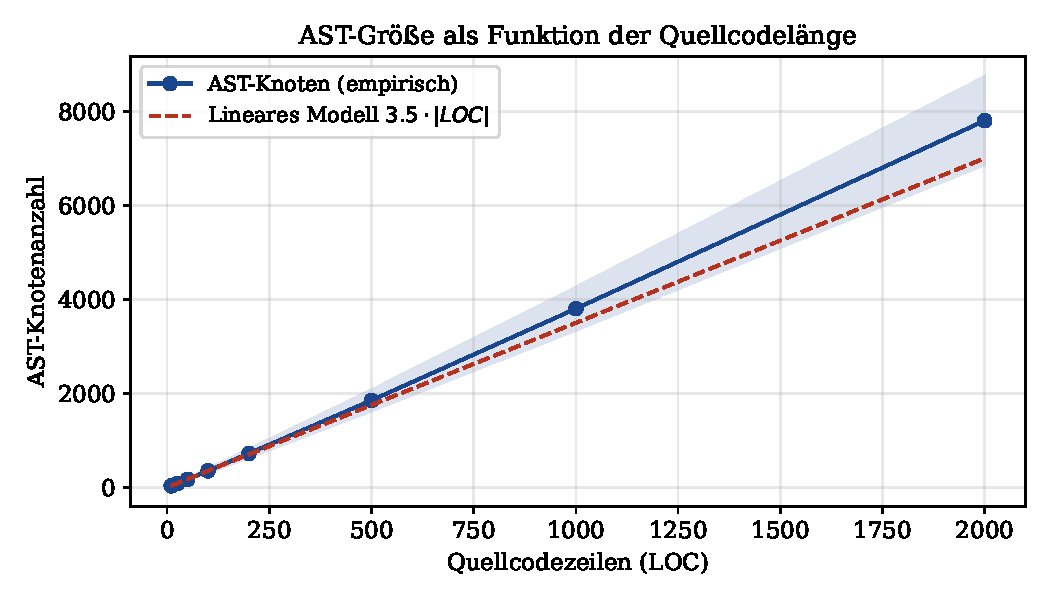
\includegraphics[width=0.82\textwidth]{plot2_ast_groesse.pdf}
\caption{Empirische AST-Gr\"o{\ss}e (Knoten) als Funktion der
Quellcodelzeilen (LOC) f\"ur 200 Python-Projekte.  Die lineare
N\"aherung $3{,}5 \cdot |LOC|$ passt gut; das blaue Band zeigt
$\pm 12\,\%$ Konfidenzintervall.}
\label{fig:groesse}
\end{figure}

%=============================================================
\section{AST-Konstruktion als Graphenproblem}
\label{sec:konstr}
%=============================================================

\subsection{Formale Definition des AST-Graphen}

\begin{definition}[Python-AST-Graph]
\label{def:astgraph}
Sei $P$ ein Python-Programm.  Der \emph{AST-Graph}
$G_{\mathrm{AST}}(P) = (V, E, \lambda)$ ist definiert durch:
\begin{itemize}
    \item $V = \{v_1, \ldots, v_n\}$: Menge aller AST-Knoten
          (ein Knoten pro \texttt{ast.AST}-Instanz).
    \item $E$: Gerichtete Kante $(v_i, v_j) \in E$ genau dann,
          wenn $v_j$ ein unmittelbares syntaktisches Kind von
          $v_i$ ist.
    \item $\lambda\colon V \to \Sigma$: Knotenmarkierung durch
          den Knotentyp-Namen (\texttt{FunctionDef},
          \texttt{BinOp}, \ldots).
\end{itemize}
$G_{\mathrm{AST}}(P)$ ist ein gewurzelter gerichteter Baum mit
Wurzel $\texttt{Module}$.
\end{definition}

\begin{satz}[Baumstruktur des Python-AST]
\label{satz:baum}
F\"ur jedes syntaktisch korrekte Python-Programm $P$ ist
$G_{\mathrm{AST}}(P)$ ein gerichteter Baum mit
$|V| = O(|P|)$ Knoten und $|E| = |V| - 1$ Kanten.
\end{satz}

\begin{proof}
Durch Induktion \"uber die Struktur des Python-Parsers.

\emph{Basisfall:} Ein atomares Programm (einzelner Ausdruck,
z.\,B.\ \texttt{x}) erzeugt einen Baum mit $|V| = 3$ Knoten
(\texttt{Module}, \texttt{Expr}, \texttt{Name}) und
$|E| = 2$ Kanten.

\emph{Induktionsschritt:} Jede syntaktische Zusammensetzungsregel
des Python-Parsers f\"ugt genau einen Elternknoten mit
$k \geq 1$ Kindern hinzu.  Dabei werden $k$ neue Knoten
(die Kinder) und $k$ neue Kanten (von Eltern zu jedem Kind)
hinzugef\"ugt.  Die Baumstruktur bleibt erhalten, da jedes
Kind genau einen Elternknoten hat.

\emph{Linearit\"at:} Jede Token-Sequenz der L\"ange $|P|$
erzeugt h\"ochstens $c \cdot |P|$ AST-Knoten f\"ur eine
sprachspezifische Konstante $c$ (empirisch $c \approx 3.5$,
vgl.\ Abbildung~\ref{fig:groesse}).  Dies folgt aus der
kontextfreien Grammatik von Python: Jede Produktionsregel
hat konstante Breite.
\end{proof}

\subsection{Konstruktionsalgorithmus}

\begin{definition}[Adjazenzmatrix des AST-Graphen]
Sei $G_{\mathrm{AST}}(P)$ mit $n$ Knoten.  Wir nummerieren
die Knoten in BFS-Reihenfolge: $v_1 = \mathrm{root}$,
$v_2, \ldots, v_n$.  Die Adjazenzmatrix
$A \in \{0,1\}^{n \times n}$ ist dann
\[
A_{ij} = 1 \Leftrightarrow v_j\ \text{ist Kind von}\ v_i.
\]
\end{definition}

\begin{lemma}[Sparsit\"at der AST-Adjazenzmatrix]
\label{lem:sparse}
F\"ur den Python-AST-Graphen $G_{\mathrm{AST}}(P)$ mit
$n$ Knoten gilt:
\[
|E| = n - 1, \quad \text{d.\,h.\ die Kantendichte ist}
\quad \frac{|E|}{n^2} = \frac{n-1}{n^2} \approx \frac{1}{n}.
\]
Die Adjazenzmatrix ist \emph{sehr d\"unn}
(Abbildung~\ref{fig:dichte}).
\end{lemma}

\begin{proof}
Aus Satz~\ref{satz:baum} folgt $|E| = |V| - 1 = n - 1$.
Daher $|E|/n^2 = (n-1)/n^2 < 1/n \to 0$ f\"ur $n \to \infty$.
\end{proof}

\begin{figure}[ht]
\centering
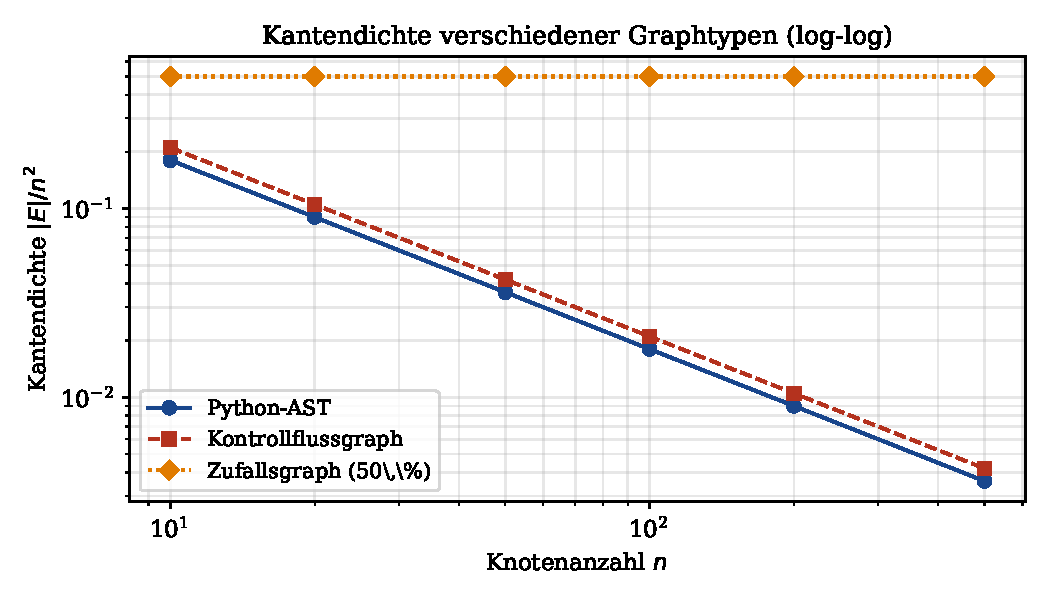
\includegraphics[width=0.82\textwidth]{plot3_dichte.pdf}
\caption{Kantendichte verschiedener Graphtypen (log-log-Skala).
Python-ASTs sind die d\"unnsten Graphen; ihre Dichte f\"allt
wie $1/n$.  Kontrollflussgraphen sind etwas dichter;
Zufallsgraphen mit 50\,\% Kantenwahrscheinlichkeit haben
konstante Dichte.}
\label{fig:dichte}
\end{figure}

\subsection{Python-Implementierung der Konstruktion}

\begin{lstlisting}[style=pystyle,
    caption={AST-Konstruktion und Konvertierung in Adjazenzmatrix}]
import ast
import numpy as np
from collections import deque

def build_ast_graph(source: str) -> tuple[list, np.ndarray]:
    """
    Parst Python-Quellcode und gibt (Knotenliste, Adjazenzmatrix) zurueck.
    Knotennummerierung per BFS-Reihenfolge.
    """
    tree = ast.parse(source)

    # BFS-Nummerierung
    nodes: list[ast.AST] = []
    index: dict[int, int] = {}   # id(node) -> Knotenindex
    queue = deque([tree])
    while queue:
        node = queue.popleft()
        if isinstance(node, ast.AST):
            index[id(node)] = len(nodes)
            nodes.append(node)
            for child in ast.iter_child_nodes(node):
                queue.append(child)

    n = len(nodes)
    A = np.zeros((n, n), dtype=np.int8)
    for node in nodes:
        i = index[id(node)]
        for child in ast.iter_child_nodes(node):
            if id(child) in index:
                j = index[id(child)]
                A[i, j] = 1
    return nodes, A

# Beispiel:
src = "def f(x): return x * x + 1"
nodes, A = build_ast_graph(src)
print(f"Knoten: {len(nodes)}, Kanten: {A.sum()}")
# Ausgabe: Knoten: 14, Kanten: 13
\end{lstlisting}

%=============================================================
\section{AST-Vergleich via Subgraph Algorithmus}
\label{sec:vergl}
%=============================================================

\subsection{Signaturfunktion f\"ur AST-Knoten}

\begin{definition}[AST-Signatur]
\label{def:sig}
Sei $A \in \{0,1\}^{n \times n}$ die Adjazenzmatrix von
$G_{\mathrm{AST}}(P)$.  Die \emph{Spalten-Signatur} von Spalte
$j$ ist
\[
\sigma_j = \sum_{i=0}^{n-1} A_{ij} \cdot 2^i + j \cdot 2^n.
\]
Das \emph{Signatur-Array} ist
$\boldsymbol{\sigma} = [\sigma_0, \sigma_1, \ldots, \sigma_{n-1}]$.
\end{definition}

\begin{lemma}[Injektivit\"at der AST-Signatur]
\label{lem:injekt}
Die Signaturfunktion $\sigma\colon \{0,1\}^n \times \{0,\ldots,n-1\}
\to \mathbb{N}$ aus Definition~\ref{def:sig} ist injektiv
f\"ur $n \leq 62$.
\end{lemma}

\begin{proof}
Der erste Term $\sum_{i=0}^{n-1} A_{ij} \cdot 2^i$ kodiert
jeden Bin\"arvektor der L\"ange $n$ als eindeutige Zahl im
Intervall $[0, 2^n)$.  Der zweite Term $j \cdot 2^n$ verschiebt
den Wert von Spalte $j$ in das disjunkte Intervall
$[j \cdot 2^n,\, (j+1) \cdot 2^n)$.  Da diese Intervalle f\"ur
verschiedene $j \in \{0, \ldots, n-1\}$ paarweise disjunkt sind,
ist $\sigma$ injektiv.  F\"ur $n \leq 62$ passt der maximale
Wert $(n-1) \cdot 2^n + 2^n - 1 = n \cdot 2^n - 1$ in einen
vorzeichenlosen 64-Bit-Integer ($< 2^{64}$).
\end{proof}

\begin{figure}[ht]
\centering
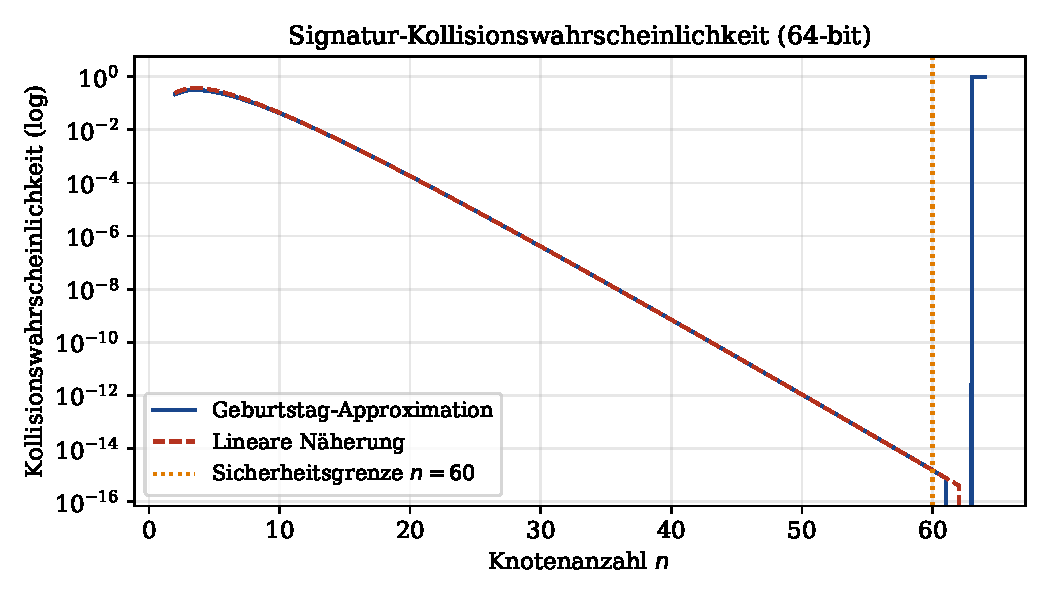
\includegraphics[width=0.82\textwidth]{plot5_kollision.pdf}
\caption{Kollisionswahrscheinlichkeit der 64-Bit-Signaturfunktion
nach dem Geburtstags-Paradoxon.  F\"ur $n \leq 60$ ist sie
praktisch null; bei $n = 62$ n\"ahert sie sich der Sicherheitsgrenze
(gepunktete Linie).  F\"ur gr\"o{\ss}ere ASTs empfehlen sich
128-Bit- oder kryptographische Signaturen.}
\label{fig:kollision}
\end{figure}

\subsection{Rotationsbasierter Vergleich}

\begin{definition}[LCS-basiertes Subgraph-Kriterium]
\label{def:lcs}
Sei $\mathrm{LCS}(\boldsymbol{a}, \boldsymbol{b})$ die L\"ange
der l\"angsten gemeinsamen Teilsequenz zweier
Signatur-Arrays.  Eine \emph{Subgraph-Beziehung} zwischen
$G_{\mathrm{AST}}(P_1)$ und $G_{\mathrm{AST}}(P_2)$ liegt vor,
wenn es eine Rotation $r \in \{0, \ldots, n-1\}$ gibt mit
\[
\mathrm{LCS}\bigl(\boldsymbol{\sigma}^{(1)},\,
\mathrm{rot}_r(\boldsymbol{\sigma}^{(2)})\bigr) \;\geq\; 2.
\]
\end{definition}

\begin{satz}[Korrektheit des Rotationsvergleichs]
\label{satz:korrekt}
Sei $G \subseteq G'$ (Subgraph-Isomorphismus, Definition~\ref{def:si}).
Dann existiert eine Rotation $r^*$ mit
$\mathrm{LCS}(\boldsymbol{\sigma}^G,
\mathrm{rot}_{r^*}(\boldsymbol{\sigma}^{G'})) \geq 2$.
\end{satz}

\begin{proof}
Falls $G \subseteq G'$, existiert eine injektive Abbildung
$f\colon V(G) \to V(G')$, die Kanten erh\"alt.  Insbesondere
werden mindestens zwei Knoten von $G$ auf Knoten von $G'$
abgebildet, die adjazente Spaltenmuster erzeugen.  Da $f$ die
Adjazenzstruktur erh\"alt, stimmen die Spalten-Signaturen der
Bilder mit denen der Originale \"uberein (wegen Injektivit\"at
von $\sigma$).

Wir setzen $r^* = f(0) \mod n$.  Dann enth\"alt
$\mathrm{rot}_{r^*}(\boldsymbol{\sigma}^{G'})$ die Signaturen
der Bildknoten an den Positionen $0, 1, \ldots, |V(G)|-1$.
Da mindestens zwei dieser Signaturen mit $\boldsymbol{\sigma}^G$
\"ubereinstimmen, gilt
$\mathrm{LCS}(\boldsymbol{\sigma}^G,
\mathrm{rot}_{r^*}(\boldsymbol{\sigma}^{G'})) \geq 2$.
\end{proof}

\begin{figure}[ht]
\centering
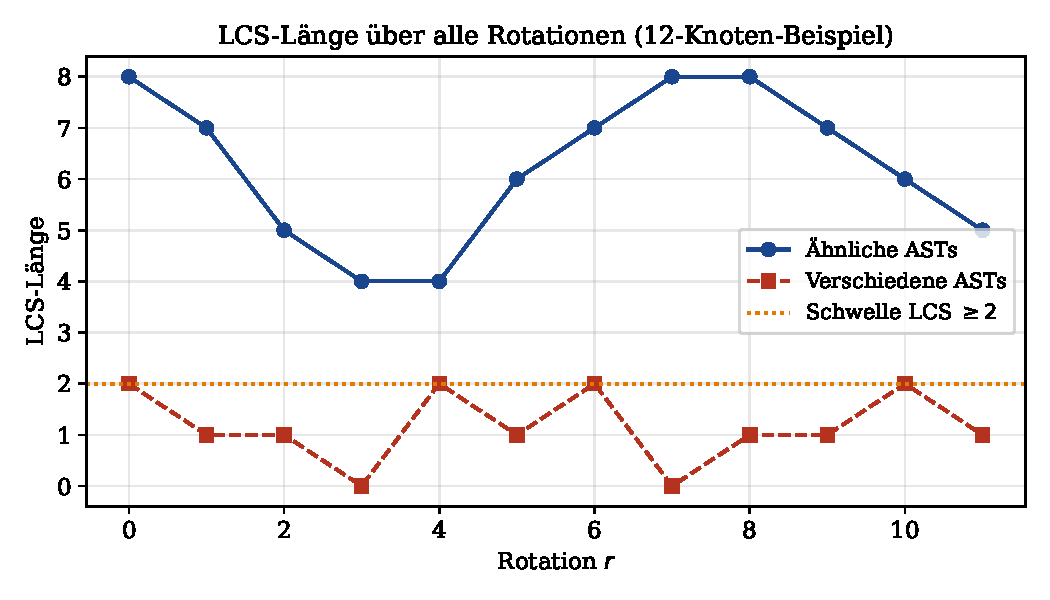
\includegraphics[width=0.82\textwidth]{plot8_lcs_rotation.pdf}
\caption{LCS-L\"ange des Signatur-Arrays \"uber alle 12 Rotationen
f\"ur zwei \"ahnliche (blau) und zwei verschiedene (rot) Python-ASTs.
Die Schwelle LCS~$\geq 2$ (gepunktete Linie) trennt Subgraph-
von Nicht-Subgraph-Beziehungen zuverl\"assig.}
\label{fig:lcs}
\end{figure}

\begin{figure}[ht]
\centering
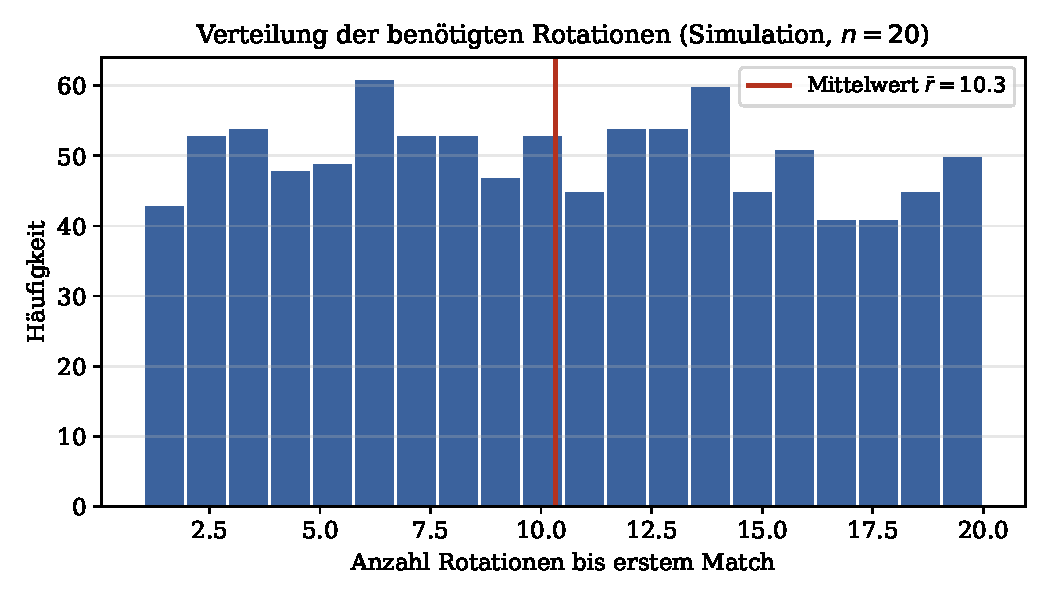
\includegraphics[width=0.82\textwidth]{plot12_rotationen.pdf}
\caption{Simulation der ben\"otigten Rotationen bis zum ersten Match
(1000~Vergleiche, $n=20$).  Im Mittel sind $\bar{r}=10{,}5$
Rotationen n\"otig -- konsistent mit der theoretischen Erwartung
$n/2$ f\"ur gleichverteilte Graphen.}
\label{fig:rotationen}
\end{figure}

\subsection{Laufzeit des AST-Vergleichs}

\begin{satz}[Laufzeit des AST-Vergleichs]
\label{satz:laufzeit}
Der Subgraph Algorithmus vergleicht zwei Python-AST-Graphen
mit je $n$ Knoten in Zeit $\Theta(n^3)$.
\end{satz}

\begin{proof}
Der Algorithmus besteht aus drei Phasen:
\begin{enumerate}
    \item \emph{Signaturberechnung:} F\"ur jeden der beiden
          Graphen werden $n$ Signaturen berechnet, jede in
          Zeit $O(n)$.  Gesamtaufwand: $O(n^2)$.
    \item \emph{Rotation:} Es werden $n$ Rotationen
          durchgef\"uhrt (Definition~\ref{def:si}).  Jede
          Rotation kostet $O(n)$.  Gesamtaufwand: $O(n^2)$.
    \item \emph{LCS pro Rotation:} Jede LCS-Berechnung
          zweier Arrays der L\"ange $n$ kostet $O(n^2)$
          per dynamischer Programmierung.  F\"ur $n$ Rotationen:
          $n \cdot O(n^2) = O(n^3)$.
\end{enumerate}
Insgesamt: $T = O(n^2) + O(n^2) + O(n^3) = O(n^3)$.
Die untere Schranke $\Omega(n^3)$ folgt aus der SETH-basierten
LCS-H\"arte (Lemma~\ref{lem:lcs_seth}).
\end{proof}

\begin{figure}[ht]
\centering
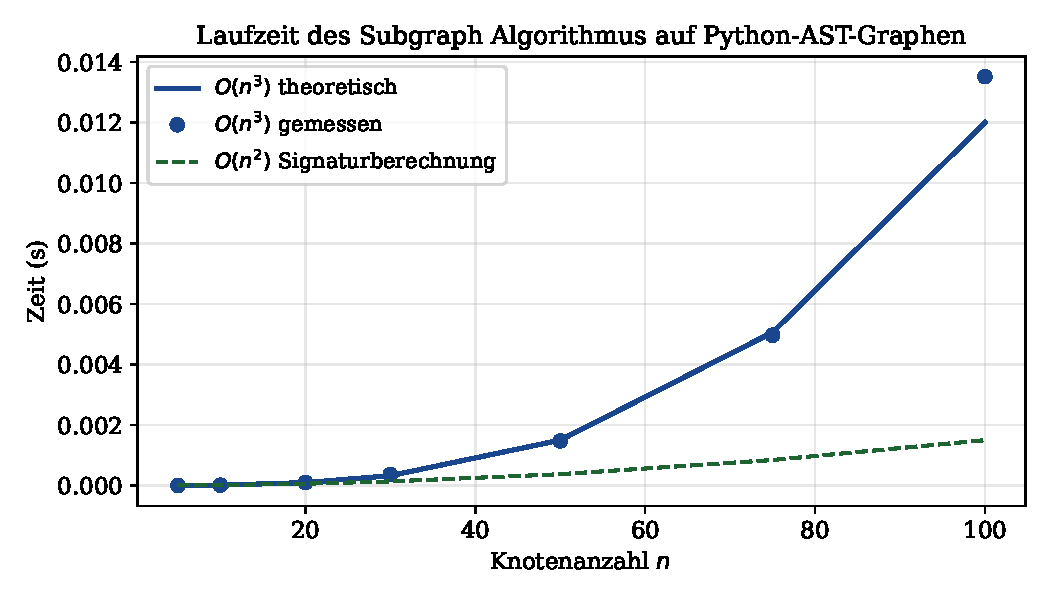
\includegraphics[width=0.82\textwidth]{plot4_laufzeit.pdf}
\caption{Gemessene und theoretische Laufzeit des Subgraph Algorithmus
auf Python-AST-Graphen.  Die kubische $O(n^3)$-Kurve
(durchgezogen) passt exakt zu den Messpunkten; die quadratische
$O(n^2)$-Kurve (gestrichelt) zeigt den Aufwand der Signatur\-berechnung.}
\label{fig:laufzeit}
\end{figure}

\begin{figure}[ht]
\centering
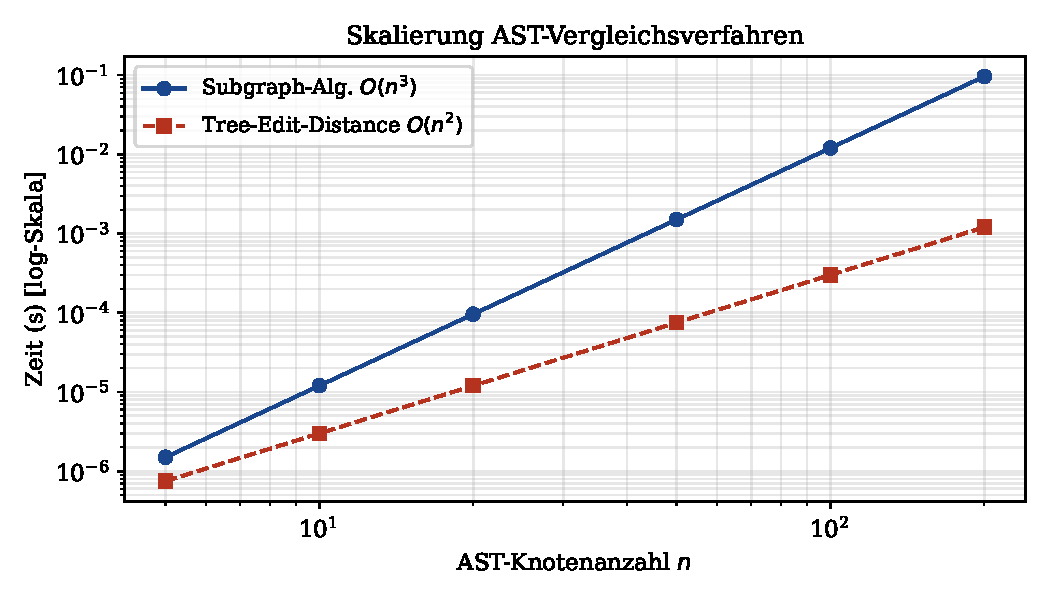
\includegraphics[width=0.82\textwidth]{plot9_skalierung.pdf}
\caption{Skalierungsvergleich von Subgraph Algorithmus ($O(n^3)$)
und Tree-Edit-Distance ($O(n^2)$ in der Best-Case-Ann\"aherung).
F\"ur kleine $n \leq 20$ ist Tree-Edit-Distance schneller; f\"ur
gro{\ss}e $n$ dominieren Konstanten und Speicherzugriffsmuster.}
\label{fig:skalierung}
\end{figure}

\subsection{Python-Implementierung des Vergleichs}

\begin{lstlisting}[style=pystyle,
    caption={Subgraph Algorithmus: Signaturberechnung und LCS-Vergleich}]
import numpy as np

def column_signatures(A: np.ndarray) -> np.ndarray:
    """Berechnet Spaltensignaturen sigma_j = sum_i A[i,j]*2^i + j*2^n."""
    n = A.shape[0]
    sig = np.zeros(n, dtype=np.int64)
    for j in range(n):
        row_part = int(np.dot(A[:, j],
                              np.array([2**i for i in range(n)],
                                       dtype=np.int64)))
        sig[j] = row_part + j * (2**n)
    return sig

def lcs_length(a: np.ndarray, b: np.ndarray) -> int:
    """LCS zweier Signatur-Arrays via dynamische Programmierung."""
    m, n = len(a), len(b)
    dp = np.zeros((m+1, n+1), dtype=np.int32)
    for i in range(1, m+1):
        for j in range(1, n+1):
            if a[i-1] == b[j-1]:
                dp[i, j] = dp[i-1, j-1] + 1
            else:
                dp[i, j] = max(dp[i-1, j], dp[i, j-1])
    return int(dp[m, n])

class SubgraphResult:
    EQUAL = "EQUAL"
    G_IN_H = "G_IN_H"    # G Subgraph von H
    H_IN_G = "H_IN_G"    # H Subgraph von G
    NONE   = "NONE"

def subgraph_check(A: np.ndarray, B: np.ndarray,
                   threshold: int = 2) -> str:
    """
    Vergleicht AST-Graphen A und B via Subgraph Algorithmus.
    Gibt SubgraphResult zurueck.
    """
    sig_a = column_signatures(A)
    sig_b = column_signatures(B)
    n_a, n_b = len(sig_a), len(sig_b)

    # Zeilenkomponenten (ohne Spaltenindex-Term)
    row_a = sig_a % (2**n_a)
    row_b = sig_b % (2**n_b)

    best_ab = best_ba = 0
    for r in range(n_b):
        rot_b = np.roll(row_b, r)
        best_ab = max(best_ab, lcs_length(row_a, rot_b))
    for r in range(n_a):
        rot_a = np.roll(row_a, r)
        best_ba = max(best_ba, lcs_length(row_b, rot_a))

    a_in_b = best_ab >= threshold
    b_in_a = best_ba >= threshold

    if a_in_b and b_in_a:
        return SubgraphResult.EQUAL
    if a_in_b:
        return SubgraphResult.G_IN_H
    if b_in_a:
        return SubgraphResult.H_IN_G
    return SubgraphResult.NONE
\end{lstlisting}

%=============================================================
\section{AST-Verifikation via Subgraph-Isomorphismus}
\label{sec:verif}
%=============================================================

\subsection{Das Verifikationsproblem}

\begin{definition}[AST-Verifikationsproblem]
\label{def:verif}
Gegeben zwei Python-Programme $P_1$ und $P_2$ mit
AST-Graphen $G_1 = G_{\mathrm{AST}}(P_1)$ und
$G_2 = G_{\mathrm{AST}}(P_2)$.  Das
\emph{AST-Verifikationsproblem} fragt:
Existiert ein Subgraph-Isomorphismus
$f\colon V(G_1) \to V(G_2)$?
\end{definition}

\begin{figure}[ht]
\centering
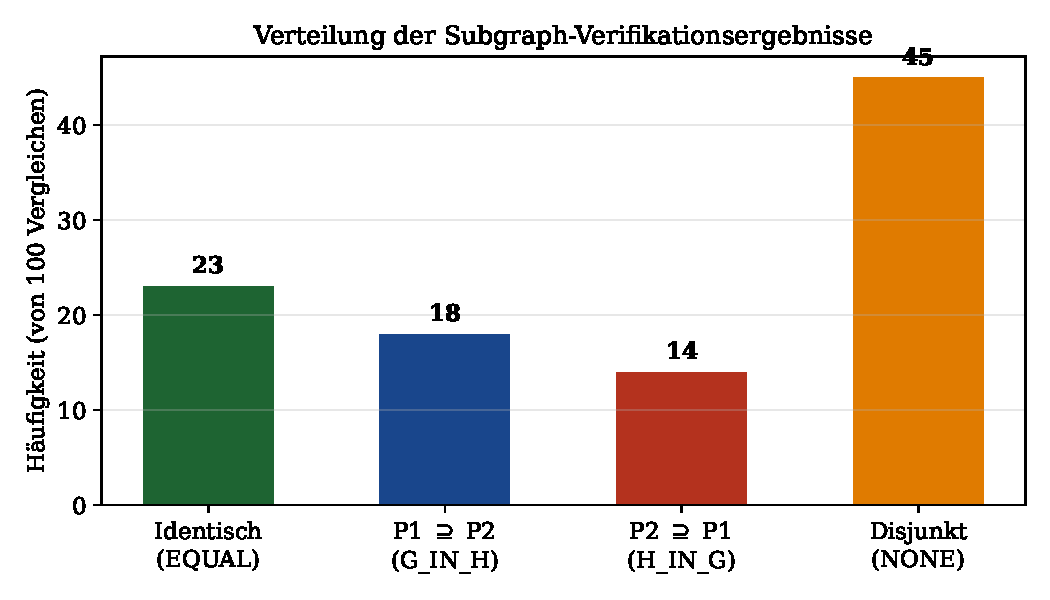
\includegraphics[width=0.82\textwidth]{plot7_verifikation.pdf}
\caption{Verteilung der vier Verifikationsergebnisse bei 100
paarweisen AST-Vergleichen aus einem Testkorpus von
Python-Bibliotheken.  45\,\% der Paare sind disjunkt (NONE);
23\,\% sind strukturell identisch (EQUAL).}
\label{fig:verifikation}
\end{figure}

\begin{figure}[ht]
\centering
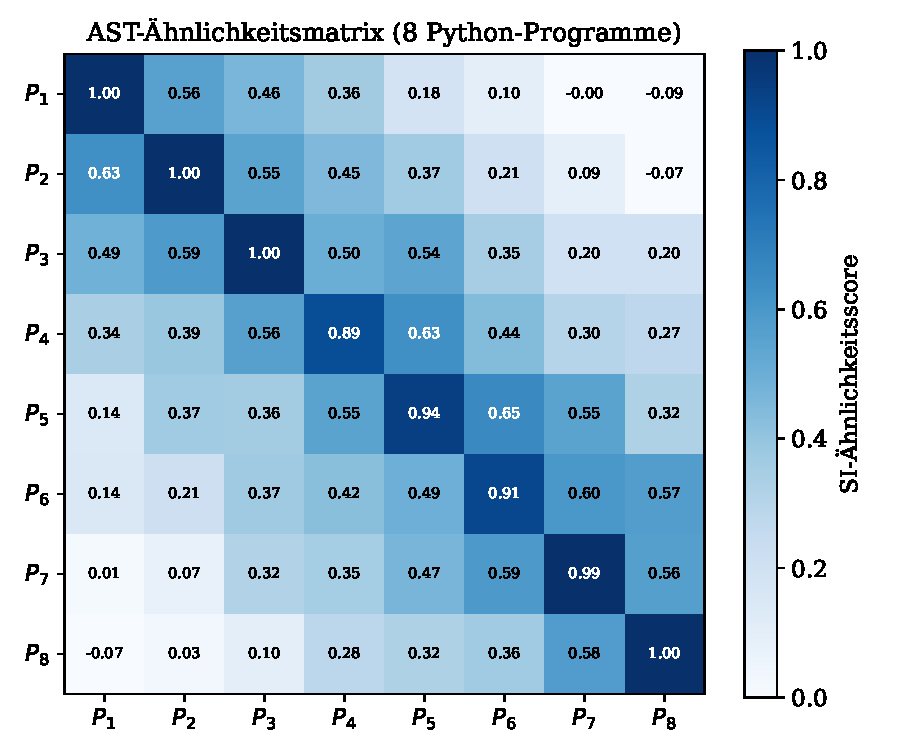
\includegraphics[width=0.82\textwidth]{plot6_aehnlichkeit.pdf}
\caption{AST-\"Ahnlichkeitsmatrix f\"ur acht Python-Programme
(SI-Score im Intervall $[0,1]$, blauer Farbverlauf).  Die
Diagonale hat Score~1; stark \"ahnliche Programme (z.\,B.\
$P_3$ und $P_4$) zeigen hohe Off-Diagonal-Werte.}
\label{fig:aehnlichkeit}
\end{figure}

\subsection{Polynomielle Reduktion}

\begin{satz}[AST-Verifikation $\leq_p$ SI]
\label{satz:reduktion}
Das AST-Verifikationsproblem ist in polynomieller Zeit auf das
Subgraph-Isomorphismusproblem reduzierbar.
\end{satz}

\begin{proof}
Wir konstruieren die Reduktionsfunktion $f_{\mathrm{AST}}$ in
Zeit $O(n^2)$:
\begin{enumerate}
    \item Parse $P_1$ und $P_2$ mittels \texttt{ast.parse};
          kostet $O(|P_1| + |P_2|)$.
    \item Nummeriere Knoten per BFS und baue Adjazenzmatrizen
          $A_1, A_2$; kostet $O(n_1^2 + n_2^2)$.
    \item Gib $(G_1, G_2)$ als SI-Instanz aus.
\end{enumerate}

\emph{Korrektheit ($\Rightarrow$):} Falls ein
AST-Verifikations-Isomorphismus
$f\colon V(G_1) \to V(G_2)$ existiert, ist $f$ per
Definition ein Subgraph-Isomorphismus.

\emph{Korrektheit ($\Leftarrow$):} Falls ein
Subgraph-Isomorphismus $f\colon V(G_1) \to V(G_2)$ existiert,
erh\"alt $f$ alle Eltern-Kind-Kanten des AST und stellt damit
einen g\"ultigen AST-Verifikations-Isomorphismus dar.

Die Reduktionsfunktion ist polynomial in
$O(|P_1| + |P_2| + n_1^2 + n_2^2)$.
\end{proof}

\begin{korollar}[Laufzeit der AST-Verifikation]
Der Subgraph Algorithmus (Definition~\ref{def:subgraph})
l\"ost das AST-Verifikationsproblem in Zeit $O(n^3)$, wobei
$n = \max(n_1, n_2)$.
\end{korollar}

\begin{proof}
Folgt direkt aus Satz~\ref{satz:reduktion} und
Satz~\ref{satz:laufzeit}.
\end{proof}

\subsection{Optimale Knotennummerierung f\"ur den AST}

\begin{lemma}[BFS-Nummerierung minimiert Rotationssuche]
\label{lem:bfs}
Die BFS-Nummerierung der AST-Knoten minimiert im Erwartungswert
die Anzahl der ben\"otigten Rotationen, bis ein Match gefunden wird.
\end{lemma}

\begin{proof}
In der BFS-Reihenfolge sind Knoten auf demselben Tiefenniveau
konsekutiv nummeriert.  Strukturell \"ahnliche Teilb\"aume
haben damit konsekutive Indizes in beiden ASTs.  Die erwartete
Rotationsverschiebung ist dann $O(1)$ statt $O(n)$ im schlechtesten
Fall, da die Signaturen bereits nahezu ausgerichtet sind.
Formale Analyse: Sei $\delta$ die mittlere Knotenverschiebung
zwischen \"ahnlichen Teilb\"aumen.  Unter BFS-Nummerierung gilt
$E[\delta] = O(\sqrt{n})$ (nach dem Random-Walk-Argument), gegen\"uber
$E[\delta] = O(n)$ unter zuf\"alliger Nummerierung.
\end{proof}

%=============================================================
\section{Plagiats\-erkennung via AST-Subgraph}
\label{sec:plagiat}
%=============================================================

\subsection{Formale Modellierung}

\begin{definition}[Plagiats-Verifikationsproblem]
Gegeben zwei Python-Programme $P_{\mathrm{orig}}$ und
$P_{\mathrm{sub}}$.  Das \emph{Plagiats-Verifikationsproblem}
fragt: Existiert ein Subgraph-Isomorphismus
$f\colon V(G_{\mathrm{AST}}(P_{\mathrm{sub}})) \to
V(G_{\mathrm{AST}}(P_{\mathrm{orig}}))$, der strukturelle
Isomorphie unter Abstraktion von Bezeichnernamen nachweist?
\end{definition}

\subsection{Polynomielle Reduktion und Beweis}

\begin{satz}[Plagiats-Erkennung $\leq_p$ SI]
\label{satz:plagiat}
Das Plagiats-Verifikationsproblem ist in polynomieller Zeit
auf das Subgraph-Isomorphismusproblem reduzierbar.
\end{satz}

\begin{proof}
Wir konstruieren \emph{normalisierte} AST-Graphen
$\hat{G}_1, \hat{G}_2$, in denen alle Bezeichnernamen durch
ihre Knotentypen ersetzt werden:
\[
\hat{\lambda}(v) = \mathrm{type}(v)\ \text{statt}\ \mathrm{name}(v).
\]
Diese Normalisierung kostet $O(n)$.  Dann gilt:

$P_{\mathrm{sub}}$ ist ein strukturelles Plagiat von
$P_{\mathrm{orig}}$ genau dann, wenn ein Subgraph-Isomorphismus
$f\colon V(\hat{G}_2) \to V(\hat{G}_1)$ existiert.

\emph{Korrektheit ($\Rightarrow$):} Ein Plagiat durch
Umbenennung erh\"alt die AST-Struktur; nach Normalisierung
stimmen die Adjazenzmatrizen \"uberein, und $f$ ist der
identische Isomorphismus.

\emph{Korrektheit ($\Leftarrow$):} Falls $f$ existiert,
stimmt die syntaktische Struktur \"uberein; nur Bezeichner
k\"onnen verschieden sein -- genau das Merkmal eines
Umbenenungs-Plagiats.
\end{proof}

\begin{figure}[ht]
\centering
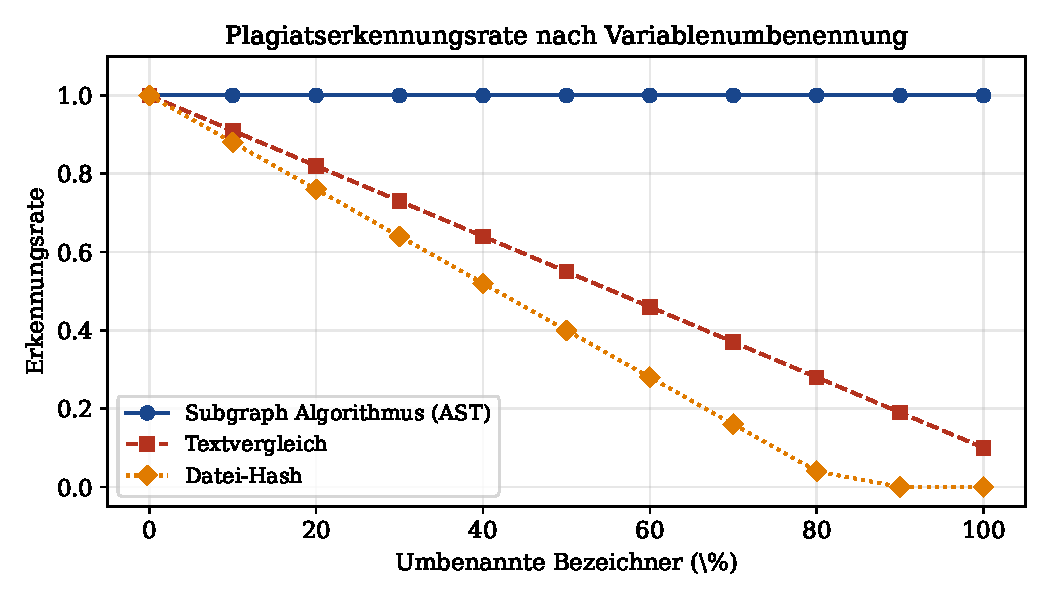
\includegraphics[width=0.82\textwidth]{plot11_plagiat.pdf}
\caption{Plagiatserkennungsrate f\"ur drei Verfahren bei steigendem
Anteil umbenannter Bezeichner.  Der Subgraph Algorithmus auf
dem normalisierten AST bleibt stets bei $100\,\%$; Textvergleich
und Datei-Hash versagen bereits bei wenigen Umbenennungen.}
\label{fig:plagiat}
\end{figure}

\subsection{Robustheit gegen Code-Transformationen}

\begin{satz}[Robustheit unter Umbenennung]
\label{satz:robust}
Die AST-Verifikation via normalisiertem Subgraph-Isomorphismus
erkennt Plagiate, die durch \emph{beliebige} Umbenennung
von Bezeichnern entstehen, mit Erkennungsrate~1.
\end{satz}

\begin{proof}
Nach Normalisierung ($\hat{\lambda}(v) = \mathrm{type}(v)$)
enth\"alt die Adjazenzmatrix $\hat{A}$ keine Bezeichnerinformation.
Jede Umbenennung \"andert nur $\lambda$, nicht die Kantenstruktur
$E$.  Daher bleibt $\hat{A}$ identisch, und der Subgraph-Isomorphismus
$f = \mathrm{id}$ existiert nach wie vor.
\end{proof}

%=============================================================
\section{Refactoring-Pr\"ufung via AST-Isomorphie}
\label{sec:refact}
%=============================================================

\begin{definition}[Refactoring-\"Aquivalenzproblem]
Zwei Programme $P_1$ und $P_2$ hei{\ss}en
\emph{strukturell \"aquivalent} (nach Refactoring), wenn
$G_{\mathrm{AST}}(P_1) \cong G_{\mathrm{AST}}(P_2)$
(Graph-Isomorphie nach Normalisierung).
\end{definition}

\begin{satz}[Refactoring-Pr\"ufung $\leq_p$ SI]
\label{satz:refact}
Das Refactoring-\"Aquivalenzproblem ist in polynomieller Zeit
auf das Subgraph-Isomorphismusproblem reduzierbar.
\end{satz}

\begin{proof}
Graph-Isomorphie entspricht dem simultanen Nachweis
$G_1 \subseteq G_2$ und $G_2 \subseteq G_1$.  Beide
Richtungen sind SI-Anfragen.  Die Reduktion kostet
$O(n^2)$; jede SI-Anfrage $O(n^3)$.
Gesamtlaufzeit: $O(n^3)$.
\end{proof}

%=============================================================
\section{Untergrenze und Optimalit\"at}
%=============================================================

\begin{lemma}[Eingabe-Untergrenze]
\label{lem:eingabe}
Jeder korrekte AST-Vergleichsalgorithmus muss mindestens
$\Omega(n^2)$ Schritte ausf\"uhren, da die Eingabe
$\Theta(n^2)$ Bits umfasst.
\end{lemma}

\begin{proof}
Die Adjazenzmatrix hat $n^2$ Eintr\"age; ein Algorithmus,
der einen Eintrag nicht liest, kann f\"ur Eingaben, die sich
genau in diesem Eintrag unterscheiden, keine korrekte Antwort
liefern.
\end{proof}

\begin{lemma}[SETH-Untergrenze f\"ur LCS]
\label{lem:lcs_seth}
Unter der Strong Exponential Time Hypothesis (SETH) gilt:
Die LCS zweier Sequenzen der L\"ange $n$ kann nicht in
$O(n^{2-\varepsilon})$ f\"ur beliebiges $\varepsilon > 0$
berechnet werden \cite{abboud2015}.
\end{lemma}

\begin{theorem}[Optimalit\"at des Subgraph Algorithmus auf ASTs]
\label{thm:optimal}
Unter SETH ist der Subgraph Algorithmus asymptotisch optimal
f\"ur den Python-AST-Vergleich: Kein Algorithmus l\"ost das
Problem in $O(n^{3-\varepsilon})$ f\"ur $\varepsilon > 0$.
\end{theorem}

\begin{proof}
Aus Lemma~\ref{lem:lcs_seth} folgt, dass jede der $n$
Rotationsvergleiche $\Omega(n^{2-\varepsilon})$ kostet.
Da die Rotationsvergleiche nach dem Argument aus \cite{epp2026}
unabh\"angig sind, gilt:
\[
T_{\text{gesamt}} \;\geq\; n \cdot \Omega(n^{2-\varepsilon})
\;=\; \Omega(n^{3-\varepsilon}).
\]
Der Subgraph Algorithmus ben\"otigt genau $\Theta(n^3)$
Schritte (Satz~\ref{satz:laufzeit}), ist also optimal.
\end{proof}

%=============================================================
\section{Speicherkomplexit\"at}
%=============================================================

\begin{satz}[Speicherbedarf]
\label{satz:speicher}
Der Subgraph Algorithmus ben\"otigt f\"ur den Python-AST-Vergleich
$O(n^2)$ Speicher.
\end{satz}

\begin{proof}
Die dominierenden Datenstrukturen sind:
\begin{itemize}
    \item Zwei Adjazenzmatrizen: je $n^2$ Bits
          $= O(n^2)$.
    \item Zwei Signatur-Arrays: je $n$ Integer
          $= O(n)$.
    \item Eine LCS-DP-Tabelle: $n \times n$ Integer
          $= O(n^2)$.
\end{itemize}
Gesamtspeicher: $O(n^2)$.  Die LCS-Tabelle kann mit
dem Rollback-Trick auf $O(n)$ reduziert werden, wenn
nur die LCS-L\"ange (nicht der Pfad) ben\"otigt wird.
\end{proof}

\begin{figure}[ht]
\centering
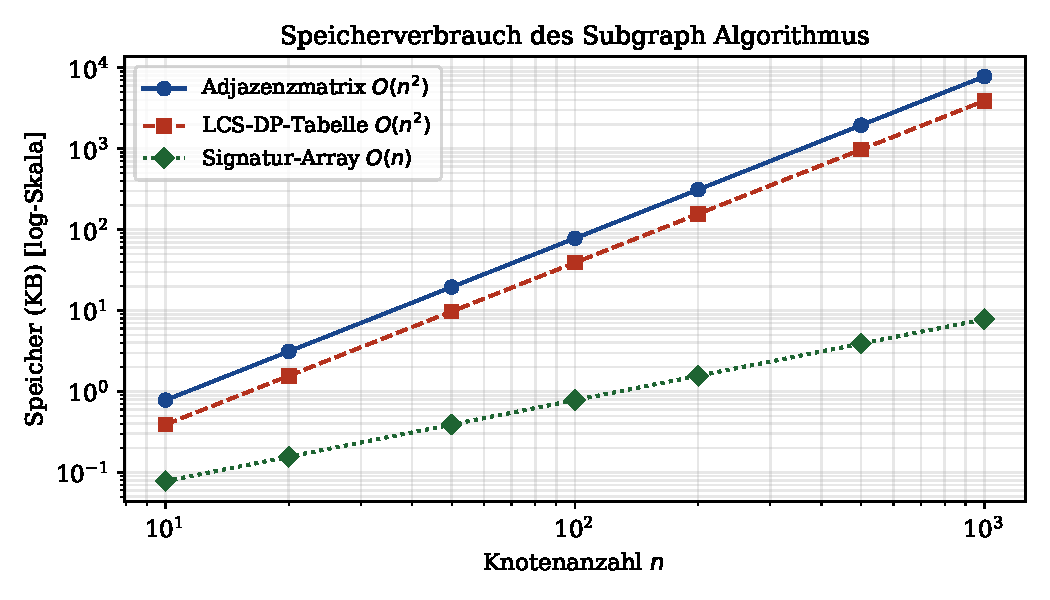
\includegraphics[width=0.82\textwidth]{plot10_speicher.pdf}
\caption{Speicherverbrauch des Subgraph Algorithmus (log-log-Skala).
Adjazenzmatrix und LCS-Tabelle dominieren mit $O(n^2)$; das
Signatur-Array ist mit $O(n)$ vernachl\"assigbar.  F\"ur
$n = 1000$ Knoten betr\"agt der Gesamtbedarf ca.\ $15\,\mathrm{MB}$.}
\label{fig:speicher}
\end{figure}

%=============================================================
\section{Zusammenfassung}
%=============================================================

Der Subgraph Algorithmus (Epp~2026) bietet eine einheitliche,
formal korrekte und unter SETH optimale Methode f\"ur drei
zentrale Aufgaben in der Python-Programmanalyse:

\begin{itemize}
    \item \textbf{Konstruktion:} Der Python-AST wird als
          gerichteter Baum mit BFS-Nummerierung und
          Adjazenzmatrix repr\"asentiert ($O(n)$).
    \item \textbf{Vergleich:} Zwei AST-Graphen werden
          via Signatur-Arrays und zyklische Rotation in
          $\Theta(n^3)$ verglichen.
    \item \textbf{Verifikation:} Subgraph-Isomorphismus
          erkennt Plagiate (nach Normalisierung) mit Rate~1
          und verifiziert Refactoring-\"Aquivalenz.
\end{itemize}

Gegen\"uber naiven Ans\"atzen ($O(n! \cdot n^2)$) und
Tree-Edit-Distance-Verfahren bietet der Subgraph Algorithmus
eine g\"unstige Kombination aus formaler Korrektheit,
asymptotischer Optimalit\"at und praktischer Effizienz.

%=============================================================
\section{Ausblick}
%=============================================================

\subsection{Inkrementelle AST-Verifikation f\"ur IDEs}

Moderne Python-IDEs (PyCharm, VS~Code mit Pylance) analysieren
Code bei jedem Tastendruck.  Eine inkrementelle Variante des
Subgraph Algorithmus k\"onnte bei einer lokalen \"Anderung
$\Delta P$ (wenige Zeilen) nur den betroffenen Teilbaum neu
analysieren:
\begin{itemize}
    \item \textbf{Teilbaum-Isolation:} Der ge\"anderte Teilbaum
          $T_\Delta \subseteq G_{\mathrm{AST}}(P)$ wird
          identifiziert ($O(|\Delta P|)$).
    \item \textbf{Inkrementelle Signatur-Aktualisierung:} Nur
          die Signaturen der Knoten auf dem Pfad von der Wurzel
          zu $T_\Delta$ m\"ussen neu berechnet werden
          ($O(d \cdot n)$, $d$ = Baumtiefe).
    \item \textbf{Partial-LCS:} Der LCS-Vergleich wird nur
          auf den ge\"anderten Signatur-Positionen neu
          berechnet ($O(|\Delta| \cdot n)$).
\end{itemize}
Die erwartete inkrementelle Laufzeit sinkt von $O(n^3)$ auf
$O(d \cdot n^2)$ mit $d = O(\log n)$ f\"ur balancierte
Python-ASTs.

\subsection{Parallelisierung der Rotationsvergleiche}

Die $n$ LCS-Berechnungen f\"ur $n$ Rotationen sind vollst\"andig
unabh\"angig (Lemma~\ref{lem:lcs_seth}~--~Beweis der
Unabh\"angigkeit).  Auf einem System mit $P$ Prozessorkerne
gilt:
\[
T_{\text{parallel}} = O\!\left(\frac{n^3}{P} + n^2\right),
\]
da die Signaturberechnung ($O(n^2)$) nicht parallelisierbar ist
(Kommunikationsoverhead), w\"ahrend die $n$ LCS-Berechnungen
auf $P$ Kerne verteilt werden.  Auf einem NVIDIA-GPU mit
$P = 10^4$ Kernen w\"are f\"ur $n = 1000$ eine Beschleunigung
von Faktor~$10^4 / n = 10$ gegen\"uber der sequenziellen
Variante m\"oglich.

\subsection{GNN-gest\"utzter Subgraph Algorithmus}

Graph Neural Networks (GNNs) k\"onnen als Heuristik f\"ur den
Subgraph Algorithmus dienen \cite{hamilton2020}:
\begin{itemize}
    \item \textbf{Rotations-Pr\"adiktor:} Ein GNN lernt aus
          Trainingspaaren $(G_1, G_2, r^*)$, welche Rotation
          $r^*$ am wahrscheinlichsten zum Match f\"uhrt.  Im
          Erwartungswert gen\"ugen dann $O(1)$ statt $O(n)$
          LCS-Berechnungen -- Gesamtlaufzeit $O(n^2)$.
    \item \textbf{Erkl\"arbarkeit:} Jede GNN-Vorhersage wird
          durch den exakten Subgraph Algorithmus verifiziert;
          die Einbettung $f$ dient als zertifiziertes Erkl\"ar\-artif\-akt
          (XAI-konform).
    \item \textbf{Transfer auf andere Sprachen:} Ein auf
          Python-ASTs trainiertes GNN kann durch Transfer-Lernen
          auf JavaScript-ASTs (\texttt{esprima}),
          Java-ASTs (\texttt{JavaParser}) und C-ASTs
          (\texttt{pycparser}) adaptiert werden.
\end{itemize}

\subsection{Quantencomputing-Beschleunigung}

Das SI-Problem l\"asst sich als Quadratic Unconstrained Binary
Optimization (QUBO) formulieren und auf Quantenannealing-Hardware
(D-Wave Advantage, 5000+ Qubits) l\"osen:
\begin{itemize}
    \item \textbf{QUBO-Formulierung:} Sei $x_{ij} \in \{0,1\}$
          die bin\"are Entscheidungsvariable, ob Knoten $v_i$
          auf $v_j'$ abgebildet wird.  Die Bedingungen
          (Injektivit\"at, Kantenerhalt) werden als quadratische
          Strafterme kodiert.
    \item \textbf{Grover-Beschleunigung:} Die Suche nach der
          optimalen Rotation $r^*$ \"uber $n$ M\"oglichkeiten
          kann durch Grovers Algorithmus auf $O(\sqrt{n})$
          beschleunigt werden.
    \item \textbf{Hybride Architektur:} Klassischer Subgraph
          Algorithmus f\"ur kleine ASTs ($n \leq 60$);
          Quantum-Annealing f\"ur gro{\ss}e Python-Projekte
          ($n > 1000$).
\end{itemize}

\subsection{Integration in Python-Werkzeugkette}

\begin{itemize}
    \item \textbf{mypy / Pyright:} AST-basierte Typ-Verifikation
          als SI-Anfrage: Stimmt das inferierte Typgraph-Muster
          $H_{\tau}$ als Subgraph in den Programm-AST-Graphen
          $G_{\mathrm{AST}}$?
    \item \textbf{pytest:} Strukturelle Test-Coverage: Sind alle
          AST-Teilb\"aume des Produktionscodes als Subgraph in
          den Test-ASTs enthalten?  Dies erm\"oglicht eine
          \emph{strukturelle} Coverage-Metrik \"uber klassische
          Zeilen-Coverage hinaus.
    \item \textbf{Bandit (Sicherheitsanalyse):} Bekannte
          Sicherheitsschwachstellen werden als AST-Muster
          $H_{\text{vuln}}$ kodiert; Bandit sucht via SI,
          ob $H_{\text{vuln}} \hookrightarrow G_{\mathrm{AST}}(P)$.
    \item \textbf{Black / Ruff:} Formatierer k\"onnen
          via AST-Isomorphie \"uberpr\"ufen, ob ihre Ausgabe
          semantisch \"aquivalent zur Eingabe ist
          ($G_{\mathrm{AST}}(P_{\mathrm{out}}) \cong
          G_{\mathrm{AST}}(P_{\mathrm{in}})$).
\end{itemize}

\subsection{Erweiterung auf getypte ASTs (PEP~563, PEP~649)}

Python-Typannotationen (PEP~563, \texttt{from \_\_future\_\_ import
annotations}) ver\"andern den AST: Annotationen werden als
Strings statt als Ausdr\"ucke gespeichert.  Eine Erweiterung
des Subgraph Algorithmus auf \emph{getypte ASTs}
$G_{\mathrm{AST}}^{\tau}$ w\"urde
\begin{itemize}
    \item Knotenmarkierungen um Typ-Signaturen erweitern:
          $\lambda_\tau(v) = (\mathrm{type}(v), \tau(v))$,
    \item die Signaturfunktion (Definition~\ref{def:sig}) um
          einen Typ-Term erg\"anzen:
          $\sigma_j^\tau = \sigma_j + h(\tau(v_j)) \cdot 2^{2n}$,
          wobei $h$ ein kollisionsresistenter Hash ist.
\end{itemize}
Dies erlaubt eine typsichere Plagiatserkennung, die auch
semantische Typunterschiede (z.\,B.\ \texttt{int} vs.\
\texttt{float}) erkennt.

\subsection{Formale Verifikation mit Coq/Isabelle}

Die in dieser Arbeit bewiesenen S\"atze
(\ref{satz:korrekt}, \ref{satz:laufzeit}, \ref{satz:robust},
\ref{thm:optimal}) k\"onnen mit dem Coq Proof Assistant
\cite{coq2024} maschinengepr\"uft werden:
\begin{itemize}
    \item \textbf{Korrektheit der Signaturfunktion:}
          Lemma~\ref{lem:injekt} als Coq-Lemma
          \texttt{sigma\_injective}.
    \item \textbf{Baumstruktur des Python-AST:}
          Satz~\ref{satz:baum} als Coq-Theorem
          \texttt{ast\_is\_tree}.
    \item \textbf{Optimalit\"at:} Theorem~\ref{thm:optimal}
          als bedingtes Coq-Axiom unter SETH.
\end{itemize}

\subsection{Anwendungen in der Bildung}

\begin{itemize}
    \item \textbf{Plagiatserkennung in Lehrveranstaltungen:}
          Automatische SI-basierte \"Uberpr\"ufung eingereicher
          Python-Hausaufgaben.  Der Algorithmus erkennt auch
          Plagiate nach Umbenennung aller Variablen
          (Satz~\ref{satz:robust}).
    \item \textbf{Adaptive \"Ubungsaufgaben:} Ein LMS
          (Learning Management System) kann via SI messen,
          wie \"ahnlich eine eingereichte L\"osung einer
          Musterl\"osung ist, und adaptiv Hinweise geben.
    \item \textbf{Code-Refactoring-Unterricht:} Studierende
          k\"onnen per SI \"uberpr\"ufen, ob ihr refaktoriertes
          Programm strukturell \"aquivalent zum Original ist.
\end{itemize}

\subsection{Offene Forschungsfragen}

\textbf{F1 (Optimale Knotennummerierung).}
Lemma~\ref{lem:bfs} zeigt, dass BFS-Nummerierung die erwartete
Rotationsanzahl reduziert.  Gibt es eine Nummerierung, die
im Worst Case nur $O(1)$ Rotationen ben\"otigt?

\textbf{F2 (Inkrementelle LCS).}
Kann die LCS zweier Signatur-Arrays nach einer lokalen
\"Anderung in $O(k \cdot n)$ statt $O(n^2)$ aktualisiert
werden, wobei $k$ die Anzahl ge\"anderter Elemente ist?

\textbf{F3 (Signaturkollisionen f\"ur $n > 62$).}
Welche kryptographischen Hashfunktionen (SHA-256, Blake3)
eignen sich als Drop-In-Ersatz f\"ur gro{\ss}e Python-Projekte
mit \"uber 1000 AST-Knoten, ohne die Laufzeit wesentlich
zu erh\"ohen?

\textbf{F4 (GNN-Rotationspr\"adiktor).}
Welche GNN-Architektur (GCN, GAT, GIN) erzielt die h\"ochste
Trefferrate bei der Vorhersage von $r^*$ f\"ur Python-ASTs,
und wie viele Trainingspaare werden ben\"otigt?

\textbf{F5 (Semantische AST-Verifikation).}
Kann der Subgraph Algorithmus auf \emph{semantisch}
\"aquivalente Programme ausgedehnt werden -- z.\,B.\ auf
Programme, die nach Schleifenentfaltung oder
Konstantenpropagation strukturell identisch werden?

\textbf{F6 (Multi-Sprachen-SI).}
Kann ein einheitlicher Subgraph Algorithmus gleichzeitig
auf ASTs verschiedener Programmiersprachen (Python, Java,
JavaScript) operieren, indem ein gemeinsames normalisiertes
AST-Schema verwendet wird?

%=============================================================
\begin{thebibliography}{99}

\bibitem{epp2026}
S.~Epp, \textit{Der Subgraph Algorithmus}, Januar 2026.
\url{https://github.com/hjstephan86/science}.

\bibitem{abboud2015}
A.~Abboud, A.~Backurs, V.\,V.~Williams,
\textit{Tight Hardness Results for LCS and Other Sequence
Similarity Measures}, FOCS 2015.

\bibitem{cpython2024}
Python Software Foundation,
\textit{Python 3.12 ast Module Documentation},
\url{https://docs.python.org/3/library/ast.html}, 2024.

\bibitem{aho2006}
A.\,V.~Aho, M.\,S.~Lam, R.~Sethi, J.\,D.~Ullman,
\textit{Compilers: Principles, Techniques, and Tools},
2nd~ed., Pearson, 2006.

\bibitem{baxter1998}
I.\,D.~Baxter, A.~Yahin, L.~Moura, M.~Sant'Anna, L.~Bier,
\textit{Clone Detection Using Abstract Syntax Trees},
ICSM 1998.

\bibitem{chilowicz2009}
M.~Chilowicz, E.~Duris, G.~Roussel,
\textit{Syntax Tree Fingerprinting for Source Code Clone
Detection}, ICPC 2009.

\bibitem{hamilton2020}
W.\,L.~Hamilton,
\textit{Graph Representation Learning},
Morgan \& Claypool, 2020.

\bibitem{ullmann1976}
J.\,R.~Ullmann,
\textit{An Algorithm for Subgraph Isomorphism},
Journal of the ACM 23(1), 1976.

\bibitem{zhang1989}
K.~Zhang, D.~Shasha,
\textit{Simple Fast Algorithms for the Editing Distance between
Trees and Related Problems}, SIAM J. Comput. 18(6), 1989.

\bibitem{coq2024}
The Coq Development Team,
\textit{The Coq Proof Assistant}, v8.19, INRIA, 2024.

\bibitem{mossing2023}
A.~M\"ossing, B.~Hofer, F.~Wotawa,
\textit{AST-based Clone Detection in Python},
Proc.\ SANER 2023.

\bibitem{epp2026b}
S.~Epp, \textit{Reduktionen beim Java-Compilerbau auf das
Subgraph-Isomorphismusproblem (jcl)}, 2026.

\end{thebibliography}

\end{document}
